\chapter{Threads e Sincronizzazione}

\section{Race Condition}

Una “concorrenza incontrollata” può portare a un comportamento non deterministico
(cioè un programma può mostrare un comportamento diverso per lo stesso insieme
di input).
Una \textit{race condition} si verifica in qualsiasi scenario in cui due (o più)
threads possono
produrre un comportamento diverso, a seconda del thread che viene eseguito per primo.
Le race conditions possono derivare da flussi di controllo affidabili o non
affidabili.\\
I \textit{flussi di controllo affidabili} (\textbf{trusted}) sono thread
strettamente correlati tra di loro che fanno parte dello stesso programma.
Invece, un \textit{flusso di controllo non affidabile} (\textbf{untrusted})
è un'applicazione o un processo separato, spesso di origine sconosciuta,
che viene eseguito in comtemporanea.\\

Tre proprietà sono necessarie perché una race conditions esista:
\begin{enumerate}
    \item \textit{Concurrency property}: Almeno due flussi di controllo
          devono essere eseguiti simultaneamente.
    \item \textit{Shared object property}: Deve esistere almeno un oggetto
          condiviso ed
          essere accessibile da
          entrambi i flussi concorrenti.
    \item \textit{Change state property} (Cambiare la proprietà di stato):
          Almeno uno dei flussi di
          controllo deve modificare lo stato dell'oggetto in condivisione.
\end{enumerate}

\subsection{Problemi delle race conditions e come eliminarle}

Le Race Conditions sono un difetto del software e sono una frequente fonte di
vulnerabilità.
Sono particolarmente insidiose perché dipendono dal timing e si manifestano
sporadicamente. Di conseguenza, sono difficili da rilevare, riprodurre ed
eliminare e possono
causare errori come la corruzione dei dati o crash.
Esse si manifestano in vari ambienti di runtime, compresi i sistemi operativi
che devono
controllare l'accesso alle risorse condivise, soprattutto attraverso la
programmazione dei vari
processi. Ci può essere concorrenza anche in presenza di un unico processore.
Da notare che è responsabilità del programmatore assicurarsi che il suo codice
sia correttamente
sequenziato, indipendentemente da come gli ambienti di runtime programmano
l'esecuzione
della programmazione.
La loro eliminazione inizia con l'identificazione delle \textit{Race Windows}.
Una race window è un
segmento di codice che accede all'oggetto condiviso in modo da aprire una
finestra di opportunità
durante la quale altri flussi concorrenti potrebbero "correre dentro" (race in)
e alterare
l'oggetto. Fondamentalmente è una zona di codice sottoposta a più flussi di
controllo.
Una race windows non è protetta da un lock o da qualsiasi altro meccanismo.
Se viene
protetta da una lock o simili viene detta “\textit{sezione critica}”.

\paragraph{Esempio.}\ \\

Gli esempi più subdoli possono dipendere anche da come è fatto il processore !
Prendiamo in considerazione il seguente codice:

\begin{figure}[H]
    \centering
    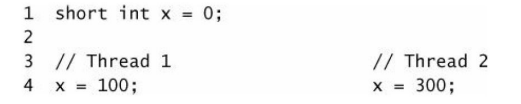
\includegraphics[width=10cm, keepaspectratio]{capitoli/secure_coding/img/cap_6/esempio1.png}
    \caption{Codice di due thread.}
\end{figure}

Come possiamo notare, i due thread assegnano un valore diverso alla stessa variabile
condivisa. Queste istruzioni
possono essere eseguite in modo diverso a livello architetturale.

\begin{figure}[H]
    \centering
    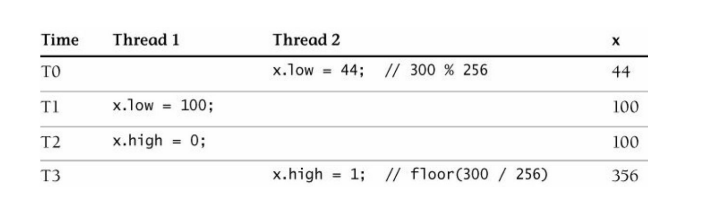
\includegraphics[width=10cm, keepaspectratio]{capitoli/secure_coding/img/cap_6/esempio1_tab.png}
    \caption{Tabella che descrive l'ordine di esecuzione delle istruzioni.}
\end{figure}

La race windows in questo caso, sono gli assegnamenti da entrambe le parti.
I registri possono essere
trattati come due metà differenti, indipendentemente dalla dimensione.
Come il compilatore
compila e come il processore si organizza è trasparente al programmatore.
Supponiamo che l'assegnamento venga effettuato in due parti da 32 bit.
Il thread 2 scrive 300, cioè $256+44$. Prima setta la parte bassa,
cioè la parte meno
significativa, a $44$; quella più significativa ad $1$.
$300$ infatti non ci sta in 8 bit.
Nel mentre però arriva il thread 1 che setta solo la parte bassa, quella meno \
significativa a $100$.
Alla fine la variabile \verb|x| conterrà il valore $100+256=356$.

\subsubsection{Race Condition su File}

Anche file e directory sono oggetti condivisi.
Le sequenze di accesso ai file in cui un file viene aperto, letto o scritto,
chiuso ed
eventualmente riaperto da funzioni separate chiamate in un certo intervallo di
tempo sono
regioni fertili per le race conditions. I file aperti sono condivisi da
peer threads, e i file system
possono essere manipolati da processi indipendenti.

\paragraph{Esempio.}\ \\

%TODO: sistemare meglio. Pagina 32.
In questo codice avviene un cambio di directory.
Dalla linea 2 poi andiamo in
\verb|/tmp/a/b| (linea 3) e così via.
C'è una race window tra le linee 4 e 6. La linea 6 consiste
praticamente nell'andare in /tmp/a/b e con la 7 si rimuove la
directory c. unlink rimuove i link da tutti i file.
Un exploit consiste nel seguente comando, se eseguito durante
questa race window: mv /tmp/a/b/c /tmp/c
In questo modo abbiamo cambiato directory: abbiamo spostato
quella in cui eravamo in tmp/c.

\section{Fuzz Testing \& Sanificazione}